\chapter{Floats (Figures, Tables, Algorithms, Etc.)}

\section{Figures}

This chapter includes the guidelines on how to properly format figures, tables, and other floats in \LaTeX. First, you must reference a figure in the document before you place it in the document. For instance, I must talk about Figure \ref{fig:1} before I place it below.
\begin{figure}[h]
	\begin{center}
		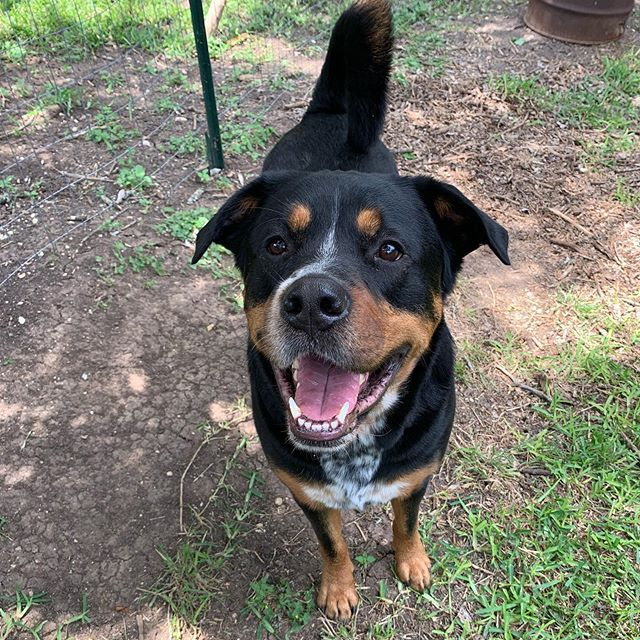
\includegraphics[scale=0.3]{einstein.jpg}
	\end{center}
\caption{This is my dog Einstein! Isn't he cute??}
\label{fig:1}
\end{figure}
\vskip -.25in
As for spacing, there must be a triple space above and below the figure. Figures must be captioned and there needs to be a double space between the figure and the caption. Captions must be positioned below the figure and are centered if one line but left aligned if more than one line. The template should take care of the centering/left-aligning but you may have to manually adjust the vertical positioning to get the double space.

Now we come to tables! Like figures, tables must be mentioned before it appears. Also like figures, there needs to be a triple space before and after the table. In tables, the caption needs to be above the table and needs to be centered no matter if it is one line or multiple lines. As for the table itself, each column needs a label. Also, there needs to be a line above the column headings, below the column headings, and at the bottom of the table, just as in Table \ref{table:2}. It has been my experience that the space between the text and the table is longer than with a figure, and so vskip/vspace commands might be needed. I had to use vskips in the document to get the spacing right.
\vskip -.07in
\begin{table}[ht]
	\centering
	\caption{Relationship between  birth and death months for 82 descendants of Queen Victoria. Birth month is the row label and death month is the column label.}
	\begin{tabular}{ccccccccccccc}
		\hline
		BM/DM & Jan & Feb & Mar & Apr & May & Jun & Jul & Aug & Sep & Oct & Nov & Dec \\  \hline
		Jan   &   1 &   0 &   0 &   0 &   1 &   2 &   0 &   0 &   1 &   0 &   1 &   0 \\ 
		Feb   &   1 &   0 &   0 &   1 &   0 &   0 &   0 &   0 &   0 &   1 &   0 &   2 \\ 
		Mar   &   1 &   0 &   0 &   0 &   2 &   1 &   0 &   0 &   0 &   0 &   0 &   1 \\ 
		Apr   &   3 &   0 &   2 &   0 &   0 &   0 &   1 &   0 &   1 &   3 &   1 &   1 \\ 
		May   &   2 &   1 &   1 &   1 &   1 &   1 &   1 &   1 &   1 &   1 &   1 &   0 \\ 
		Jun   &   2 &   0 &   0 &   0 &   1 &   0 &   0 &   0 &   0 &   0 &   0 &   0 \\ 
		Jul   &   2 &   0 &   2 &   1 &   0 &   0 &   0 &   0 &   1 &   1 &   1 &   2 \\ 
		Aug   &   0 &   0 &   0 &   3 &   0 &   0 &   1 &   0 &   0 &   1 &   0 &   2 \\ 
		Sep   &   0 &   0 &   0 &   1 &   1 &   0 &   0 &   0 &   0 &   0 &   1 &   0 \\ 
		Oct   &   1 &   1 &   0 &   2 &   0 &   0 &   1 &   0 &   0 &   1 &   1 &   0 \\ 
		Nov   &   0 &   1 &   1 &   1 &   2 &   0 &   0 &   2 &   0 &   1 &   1 &   0 \\ 
		Dec   &   0 &   1 &   1 &   0 &   0 &   0 &   1 &   0 &   0 &   0 &   0 &   0 \\  \hline
	\end{tabular}
	\label{table:2}
\end{table}
\vskip -.22in
Lastly, you may have an algorithm in your work. They follow the same general rules as a figure.

\begin{algorithm}[H]
	\SetAlgoLined
	\KwData{this text}
	\KwResult{how to write algorithm with \LaTeX2e }
	initialization\;
	\While{not at end of this document}{
		read current\;
		\eIf{understand}{
			go to next section\;
			current section becomes this one\;
		}{
			go back to the beginning of current section\;
		}
	}
	\caption{How to write algorithms}
\end{algorithm}


